\documentclass[11pt]{article}
\usepackage{euscript}
\usepackage{amsmath}
\usepackage{amsthm}
\usepackage{amssymb}
\usepackage{epsfig}
\usepackage{xspace}
\usepackage{amsmath,amssymb,amsthm}
\usepackage{graphicx}
\usepackage[margin=1in]{geometry}
\usepackage{fancyhdr}
\usepackage{color}
\usepackage{url}
\usepackage{bbm}
%%%%%%%%%%%%%%%%%%%%%%%%%%%%%%%%%
\setlength{\textheight}{9in}
\setlength{\topmargin}{-0.600in}
\setlength{\headheight}{0.2in}
\setlength{\headsep}{0.250in}
\setlength{\footskip}{0.5in}
\flushbottom
\setlength{\textwidth}{6.5in}
\setlength{\oddsidemargin}{0in}
\setlength{\evensidemargin}{0in}
\setlength{\columnsep}{2pc}
\setlength{\parindent}{1em}
\setlength{\parindent}{0pt}
\setlength{\parskip}{5pt plus 1pt}
\setlength{\headheight}{13.6pt}
%%%%%%%%%%%%%%%%%%%%%%%%%%%%%%%%%
\usepackage{epsfig}
\usepackage{xspace}
\usepackage{amsmath,amssymb,amsthm}
\usepackage{graphicx}
\usepackage[margin=1in]{geometry}
\usepackage{fancyhdr}
\usepackage{color}
\usepackage{url}
%%%%%%%  For drawing trees  %%%%%%%%%
\usepackage{tikz}
\usetikzlibrary{calc, shapes, backgrounds}
%%%%%%%%%%%%%%%%%%%%%%%%%%%%%%%%%
\setlength{\textheight}{9in}
\setlength{\topmargin}{-0.600in}
\setlength{\headheight}{0.2in}
\setlength{\headsep}{0.250in}
\setlength{\footskip}{0.5in}
\flushbottom
\setlength{\textwidth}{6.5in}
\setlength{\oddsidemargin}{0in}
\setlength{\evensidemargin}{0in}
\setlength{\columnsep}{2pc}
\setlength{\parindent}{1em}
\setlength{\parindent}{0pt}
\setlength{\parskip}{5pt plus 1pt}
\setlength{\headheight}{13.6pt}
%%%%%%%%%%%%%%%%%%%%%%%%%%%%%%%%%
\newcommand{\eps}{\varepsilon}
\renewcommand{\c}[1]{\ensuremath{\EuScript{#1}}}
\renewcommand{\b}[1]{\ensuremath{\mathbb{#1}}}
\renewcommand{\theenumi}{\alph{enumi}}
\newcommand{\s}[1]{\textsf{#1}}
\newcommand{\E}{\textbf{\textsf{E}}}
\renewcommand{\Pr}{\textbf{\textsf{Pr}}}
\newcommand\question[2]{\vspace{.25in}\hrule\textbf{#1: #2}\vspace{.5em}\hrule\vspace{.10in}}
\renewcommand\part[1]{\vspace{.10in}\textbf{(#1)}}
\newcommand\algorithm{\vspace{.10in}\textbf{Algorithm: }}
\newcommand\correctness{\vspace{.10in}\textbf{Correctness: }}
\newcommand\runtime{\vspace{.10in}\textbf{Running time: }}
\pagestyle{fancyplain}

\usepackage{listings}
\usepackage{color}

\definecolor{dkgreen}{rgb}{0,0.6,0}
\definecolor{gray}{rgb}{0.5,0.5,0.5}
\definecolor{mauve}{rgb}{0.58,0,0.82}

\lstset{frame=tb,
  language=Python,
  aboveskip=3mm,
  belowskip=3mm,
  showstringspaces=false,
  columns=flexible,
  basicstyle={\small\ttfamily},
  numbers=none,
  numberstyle=\tiny\color{gray},
  keywordstyle=\color{blue},
  commentstyle=\color{dkgreen},
  stringstyle=\color{mauve},
  breaklines=true,
  breakatwhitespace=true,
  tabsize=3
}

\graphicspath{ {.} }

\lhead{\textbf{\NAME\ (\UNI)}}
\chead{\textbf{HW\HWNUM}}
\rhead{COMS W4721, \today}


\newcommand\NAME{Daniel Kronovet}  
\newcommand\UNI{003349897}    
\newcommand\HWNUM{05}          

\begin{document}

%%%%%%%%%%%%%%%%%%%%%%%%%%%%%%%%%%%%%%%%%%%%%%%%%%%%
%%%%%%%%%%%%%%%%%%%%%%%%%%%%%%%%%%%%%%%%%%%%%%%%%%%%
%%%%%%%%%%%%%%%%%%%%%%%%%%%%%%%%%%%%%%%%%%%%%%%%%%%%

\section*{Problem 1 (Markov Chains)}

\subsection*{Part 1}

Use $w_t$ to rank the teams by sorting in decreasing value according to this vector. List the top 20 teams and their corresponding values in $w_t$ for $t = {10, 100, 200, 1000}$.

\begin{table}[!th]
\centering
\begin{tabular}{|l|c|cl}
\hline
Team & Value \\
\hline
UW-Whitewater & 0.0153227778802 \\
MountUnion & 0.0130742707022 \\
ColoradoSt-Pueblo & 0.010261008372 \\
OhioState & 0.00900979434094 \\
Linfield & 0.00878443452911 \\
MinnSt-Mankato & 0.00821200630016 \\
Wartburg & 0.00801802217138 \\
Wesley & 0.00748839125774 \\
SouthernOregon & 0.00744005399386 \\
Oregon & 0.0071542337095 \\
Alabama & 0.00714054428404 \\
NorthDakotaSt & 0.00669991126614 \\
TCU & 0.00645504966615 \\
MaryHardin-Baylor & 0.00597635138467 \\
FloridaSt & 0.005944344405 \\
Hobart & 0.00590135339447 \\
JohnCarroll & 0.00586308936461 \\
MarianIN & 0.00580349073704 \\
Widener & 0.00578632328033 \\
Concord & 0.00568551087686 \\
\hline
\end{tabular}
\caption{Teams and values for t=10}
\label{ex:table}
\end{table}

\begin{table}[!th]
\centering
\begin{tabular}{|l|c|cl}
\hline
Team & Value \\
\hline
UW-Whitewater & 0.0292759841104 \\
OhioState & 0.0276631131678 \\
Oregon & 0.0227262816528 \\
Alabama & 0.0186769498344 \\
TCU & 0.0183015022646 \\
MountUnion & 0.0168714020987 \\
FloridaSt & 0.0146308745614 \\
MichiganSt & 0.0130287913339 \\
ColoradoSt-Pueblo & 0.012999116209 \\
SouthernOregon & 0.0124931074259 \\
Baylor & 0.0122206343863 \\
GeorgiaTech & 0.0118210801366 \\
Wartburg & 0.0106811487305 \\
UCLA & 0.0106652138505 \\
Mississippi & 0.0103657540733 \\
CarrollMT & 0.0102792997905 \\
Georgia & 0.0101168632625 \\
Arizona & 0.00994307528077 \\
ArizonaSt & 0.00912162056362 \\
MississippiSt & 0.0090671268847 \\
\hline
\end{tabular}
\caption{Teams and values for t=100}
\label{ex:table}
\end{table}

\begin{table}[!th]
\centering
\begin{tabular}{|l|c|cl}
\hline
Team & Value \\
\hline
OhioState & 0.0363316355665 \\
Oregon & 0.0298306907239 \\
Alabama & 0.0243530549619 \\
TCU & 0.0240409405987 \\
FloridaSt & 0.0191361282377 \\
UW-Whitewater & 0.0182123273704 \\
MichiganSt & 0.0169569400722 \\
Baylor & 0.0160206375044 \\
GeorgiaTech & 0.0154243558734 \\
UCLA & 0.0139841818668 \\
Mississippi & 0.0134738824039 \\
Georgia & 0.0130837202891 \\
Arizona & 0.0130263839136 \\
ArizonaSt & 0.0119023046243 \\
MississippiSt & 0.0117965208801 \\
Missouri & 0.0111035953543 \\
Clemson & 0.0104986782094 \\
SouthernCal & 0.0104490838612 \\
Wisconsin & 0.0104461197528 \\
Auburn & 0.0102624439426 \\
\hline
\end{tabular}
\caption{Teams and values for t=200}
\label{ex:table}
\end{table}

\begin{table}[!th]
\centering
\begin{tabular}{|l|c|cl}
\hline
Team & Value \\
\hline
OhioState & 0.0473971919558 \\
Oregon & 0.0387971225418 \\
Alabama & 0.0316777096693 \\
TCU & 0.0313994942541 \\
FloridaSt & 0.0249885243121 \\
MichiganSt & 0.0219768459681 \\
Baylor & 0.0208884123061 \\
GeorgiaTech & 0.0201149670139 \\
UCLA & 0.0181695841427 \\
Mississippi & 0.0174792512804 \\
Georgia & 0.0169436471106 \\
Arizona & 0.0168959738481 \\
ArizonaSt & 0.0154034382393 \\
MississippiSt & 0.0153259619966 \\
Missouri & 0.014157805926 \\
Clemson & 0.0136641097675 \\
SouthernCal & 0.013544901098 \\
Wisconsin & 0.0133728015051 \\
Auburn & 0.0133087636274 \\
Utah & 0.0129390741129 \\
\hline
\end{tabular}
\caption{Teams and values for t=1000}
\label{ex:table}
\end{table}

\subsection*{Part 2}

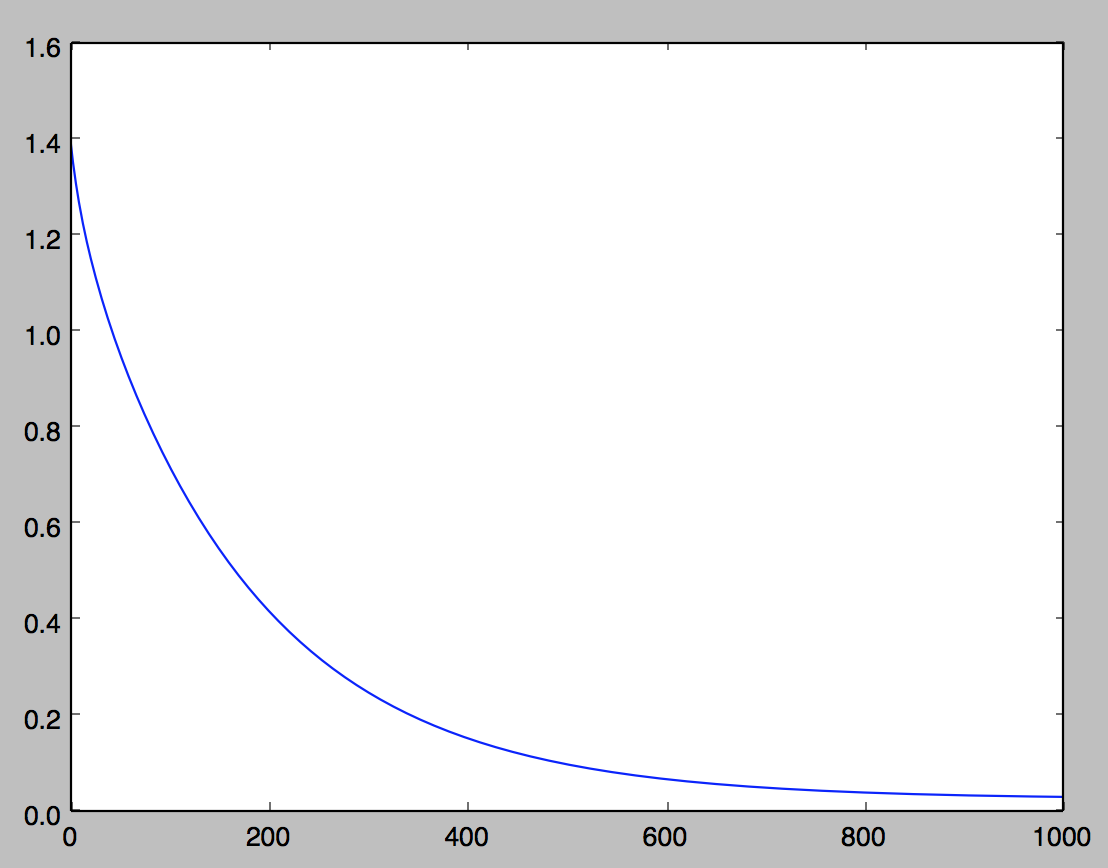
\includegraphics[scale=.5]{images/mm_eigdiff}

$||w_t - u_{1_{norm}}||_1$ as a function of $t$

At $t_1000$, $||w_t - u_{1_{norm}}||_1 =  0.031538506048135205$



\section*{Problem 2 (Nonnegative Matrix Factorization)}

\subsection*{Part 1, faces}

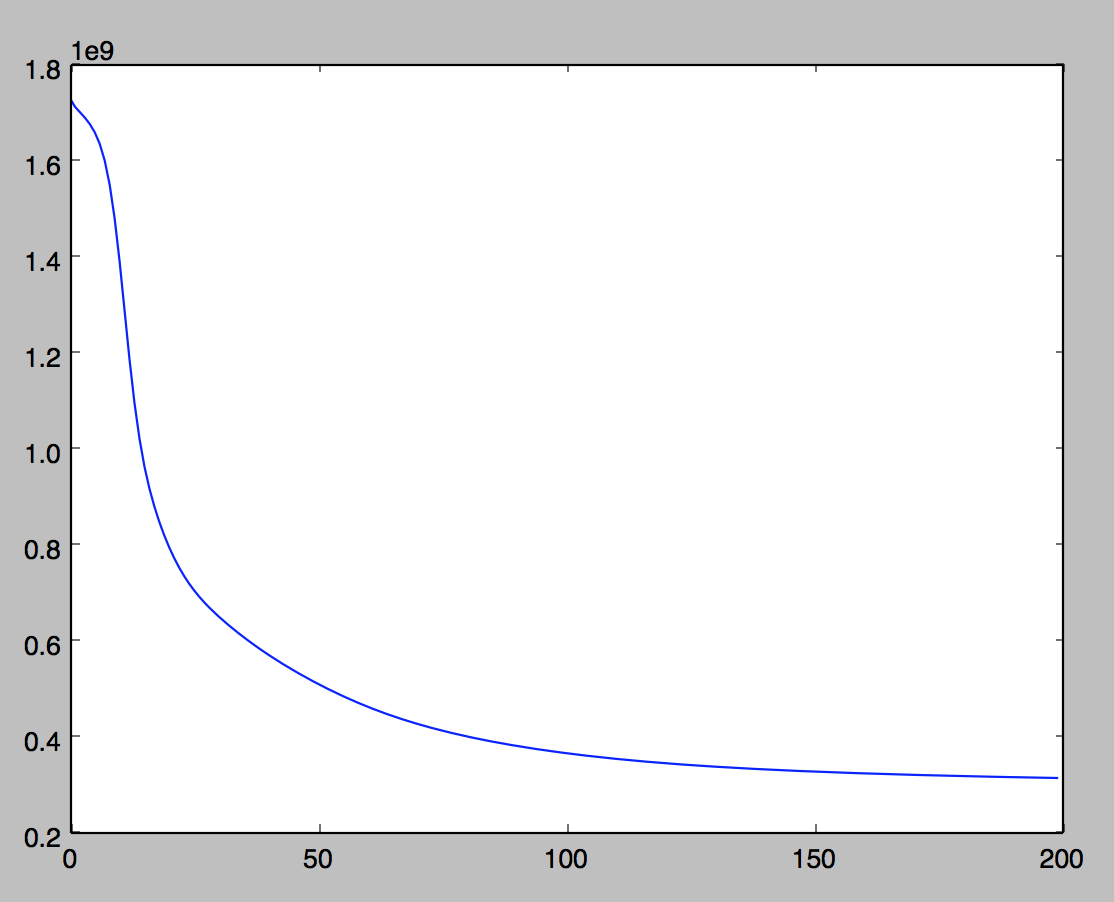
\includegraphics[scale=.5]{images/obj_euc}

Objective function for the Euclidean penalty, as function of iteration


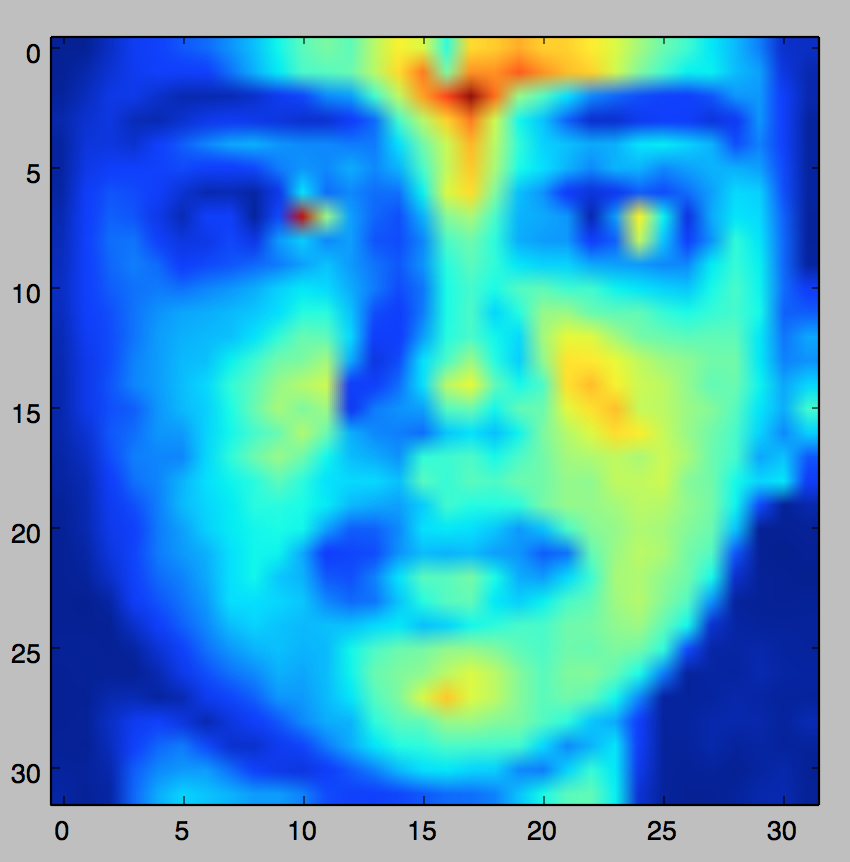
\includegraphics[scale=.5]{images/img1}

Image 1

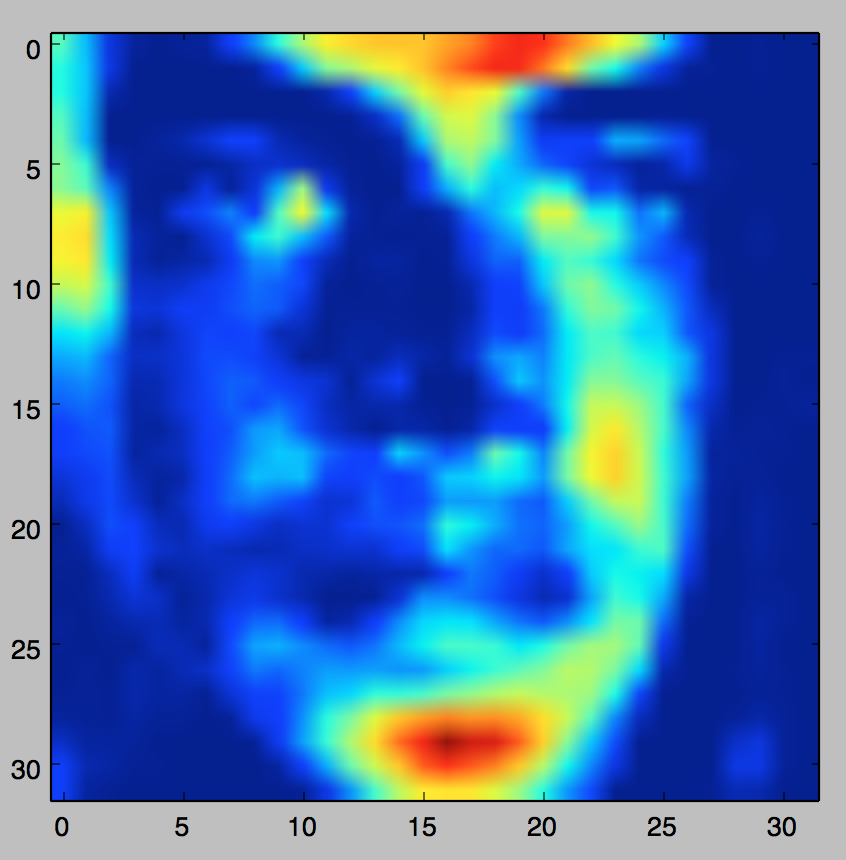
\includegraphics[scale=.5]{images/img1_W19}

$W_{19}$, corresponding to biggest value in H for image 1.

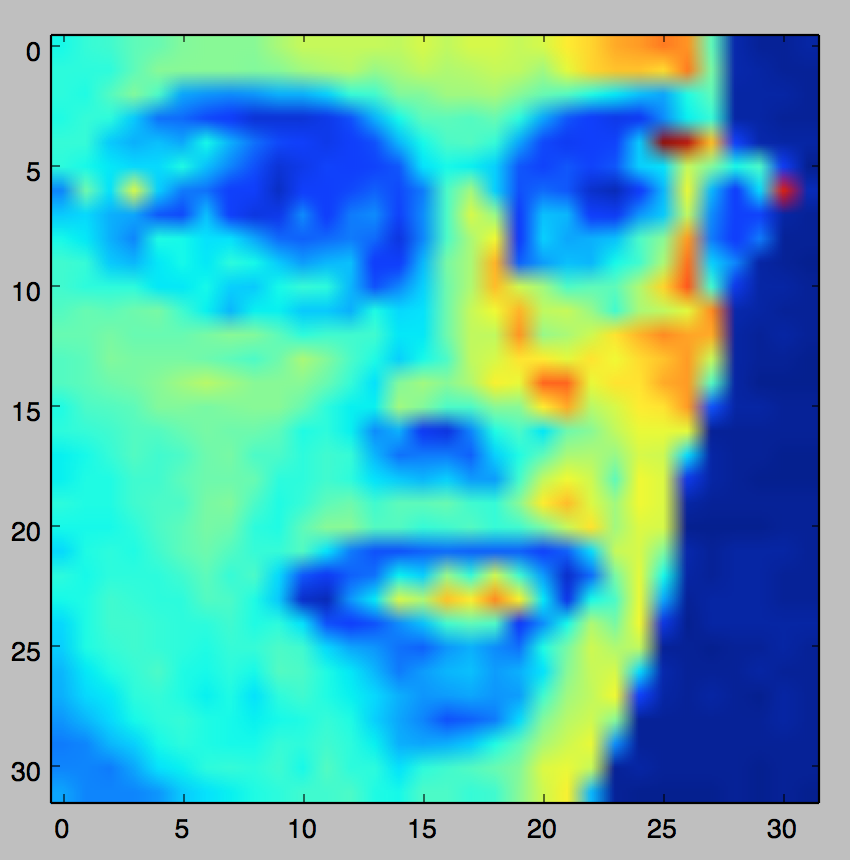
\includegraphics[scale=.5]{images/img20}

Image 20

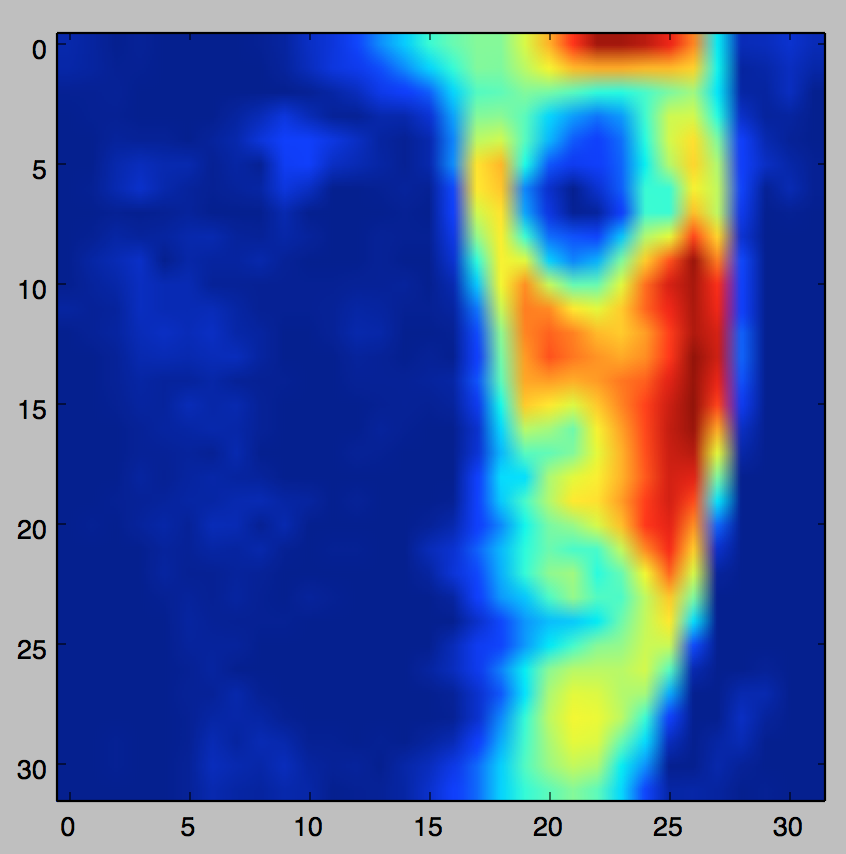
\includegraphics[scale=.5]{images/img20_W21}

$W_{21}$, corresponding to biggest value in H for image 20.

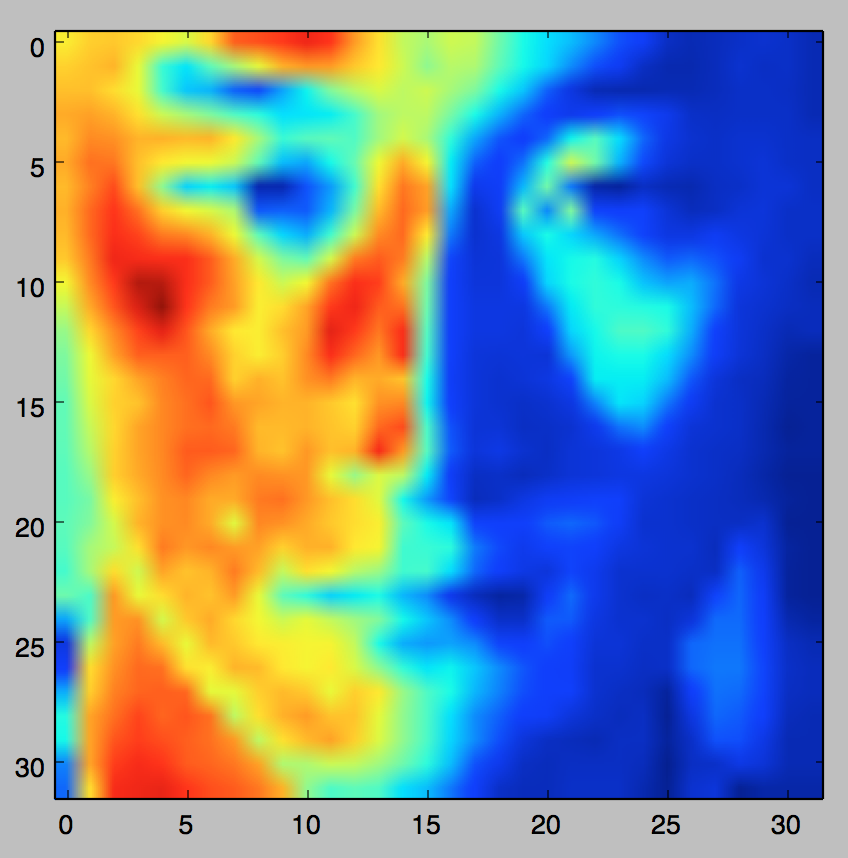
\includegraphics[scale=.5]{images/img500}

Image 500

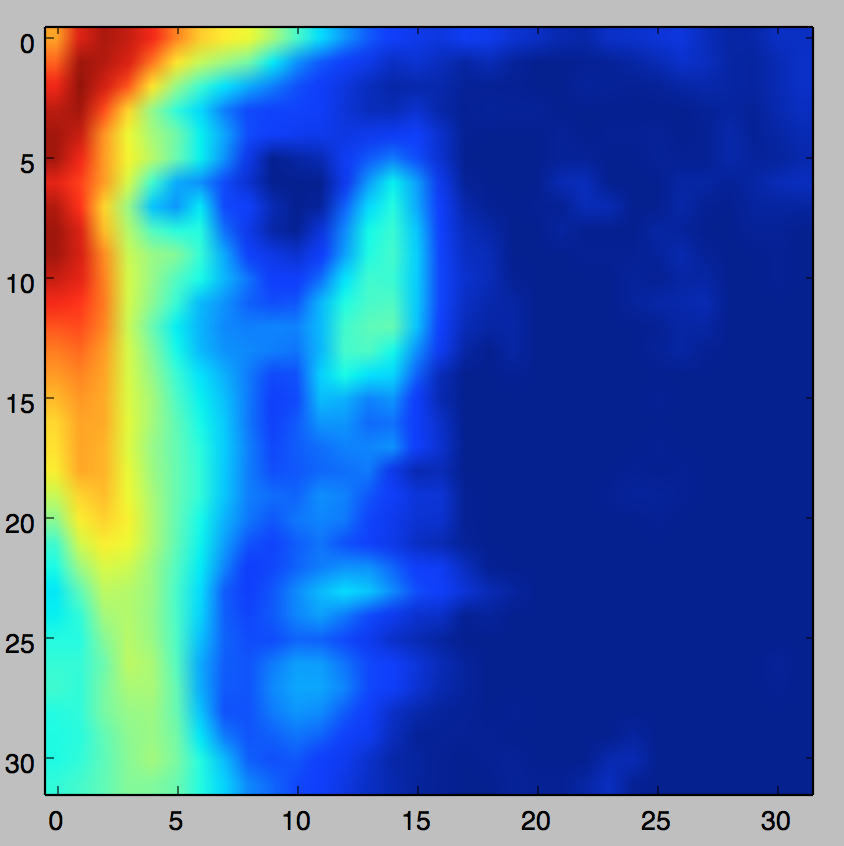
\includegraphics[scale=.5]{images/img500_W10}

$W_{10}$, corresponding to biggest value in H for image 500.

\subsection*{Part 2, documents}

\end{document}
